\chapter{\label{ch:EventLocation}Events and Event Location}

\chapauthor{Darrel J. Conway}{Thinking Systems, Inc.}

\section{Introduction}

GMAT provides a capability to determine precise epochs for important physical events along a modeled trajectory.  Examples of these events are shadow entry and exit, station rise and set, and other time-based quantities like the light time offset transmission and turn around of a tracking signal. Some of these quantities can be further processed to determine eclipse and station contact durations and similar time span quantities associated with detected event pairs.  GMAT's mathematical specification\cite{mathSpec} defines the event detection algorithm in some detail.  This chapter describes the software components that implement that algorithm.

\section{Components that Control Event Processing}

Event location in GMAT is controlled through interactions between five types of objects, and their interactions with the objects comprising the simulation designed by the user.  The five objects that work together to perform event location for these modelled objects are a propagation enabled command, a propagator contained in a PropSetup object, one or more Event objects, an EventManager, and a RootLocator.  These components play the following roles in the event location process:

\begin{itemize}
\item \textbf{Propagation Enabled Command}:  Provides the mission control sequence interfaces for event location.  Event locating is performed during execution of a propagation enabled command.  (Event evaluation can also be performed through parameter calculations tailored to report data from specific event objects.)
\item \textbf{PropSetup}:  Provides the propagator used to search for the event location.  Any GMAT propagator can be used in this context, including (once coded) ephemeris interpolators.
\item \textbf{Events}:  One or more objects responsible for providing calculations used to evaluate a measure of the desired event.  The Event objects all provide an Evaluate method that generates one or more Real values.  The values calculated in the Evaluate method are function values that evaluate to 0.0 at the epoch of the event, and that pass smoothly through zero as the data used in the evaluation are propagated through the time interval containing the event.
\item \textbf{Event Manager}: Acts as a mediator to control data interactions between the Event objects and the other components involved in the location process.
\item \textbf{Root Locator}: Manages the details of the propagation or interpolation needed to precisely locate the events on the mission timeline.
\end{itemize}

Event location is used in two distinct settings in GMAT.  During a typical mission run, users can script specific events that they would like to track for the purposes of reporting and analysis.  GMAT's propagation subsystem provides a mechanism to watch for these events as the mission is run, and locates the resulting events as they are encountered, tracking their location for the user.  Event location is also performed in the estimation subsystem, so that measurement corrections that require propagation to manage detailed precision calculation can find and propagate to the epochs for those events during the correction process.

GMAT manages two types of events: discrete events that occur at a single instant of time, and interval events that occur over a span of time.  In both cases, the epochs associated with the events are detected through zero crossings of a function.  Interval events track the start and end time for the event, and can be used to calculate the interval of time over which the event occurred.  For interval events, the event is deemed to be occurring while the event function provides a positive value.  Interval events that provide more than one Real value on event evaluation track the event span through the first event function evaluated; in other words, the first function value should be positive -- and all event criteria met -- while the interval event is happening.

This chapter presents the design for the former application.  Event processing during estimation follows the same process as generic event location, with a few additional steps required to synchronize the measurement models with the event location data.  The estimation based event location refinements are presented in Chapter~\ref{ch:MeasurementCorrections}.

\section{The Event Location Process}

Figure~\ref{fig:EventLocationSD} shows the details of the event location process.  Events that need to be located are registered with the propagation enabled command in the PrepareToPropagate() method prior to execution of the command.  At this point the EventManager evaluates each active Event and stores the event data so that the pre-propagation event state is known.  The propagation enabled command then takes a propagation step.  After the step has been taken, the EventManager again evaluates each event, and uses the results of that evaluation to determine if the event has a zero crossing or extremum in the propagation interval.  If no such trigger has occurred, the command continues processing -- either by taking additional propagation steps, or by exiting, returning control to the Sandbox so that the mission control sequence can continue executing.

\begin{figure}
\begin{center}
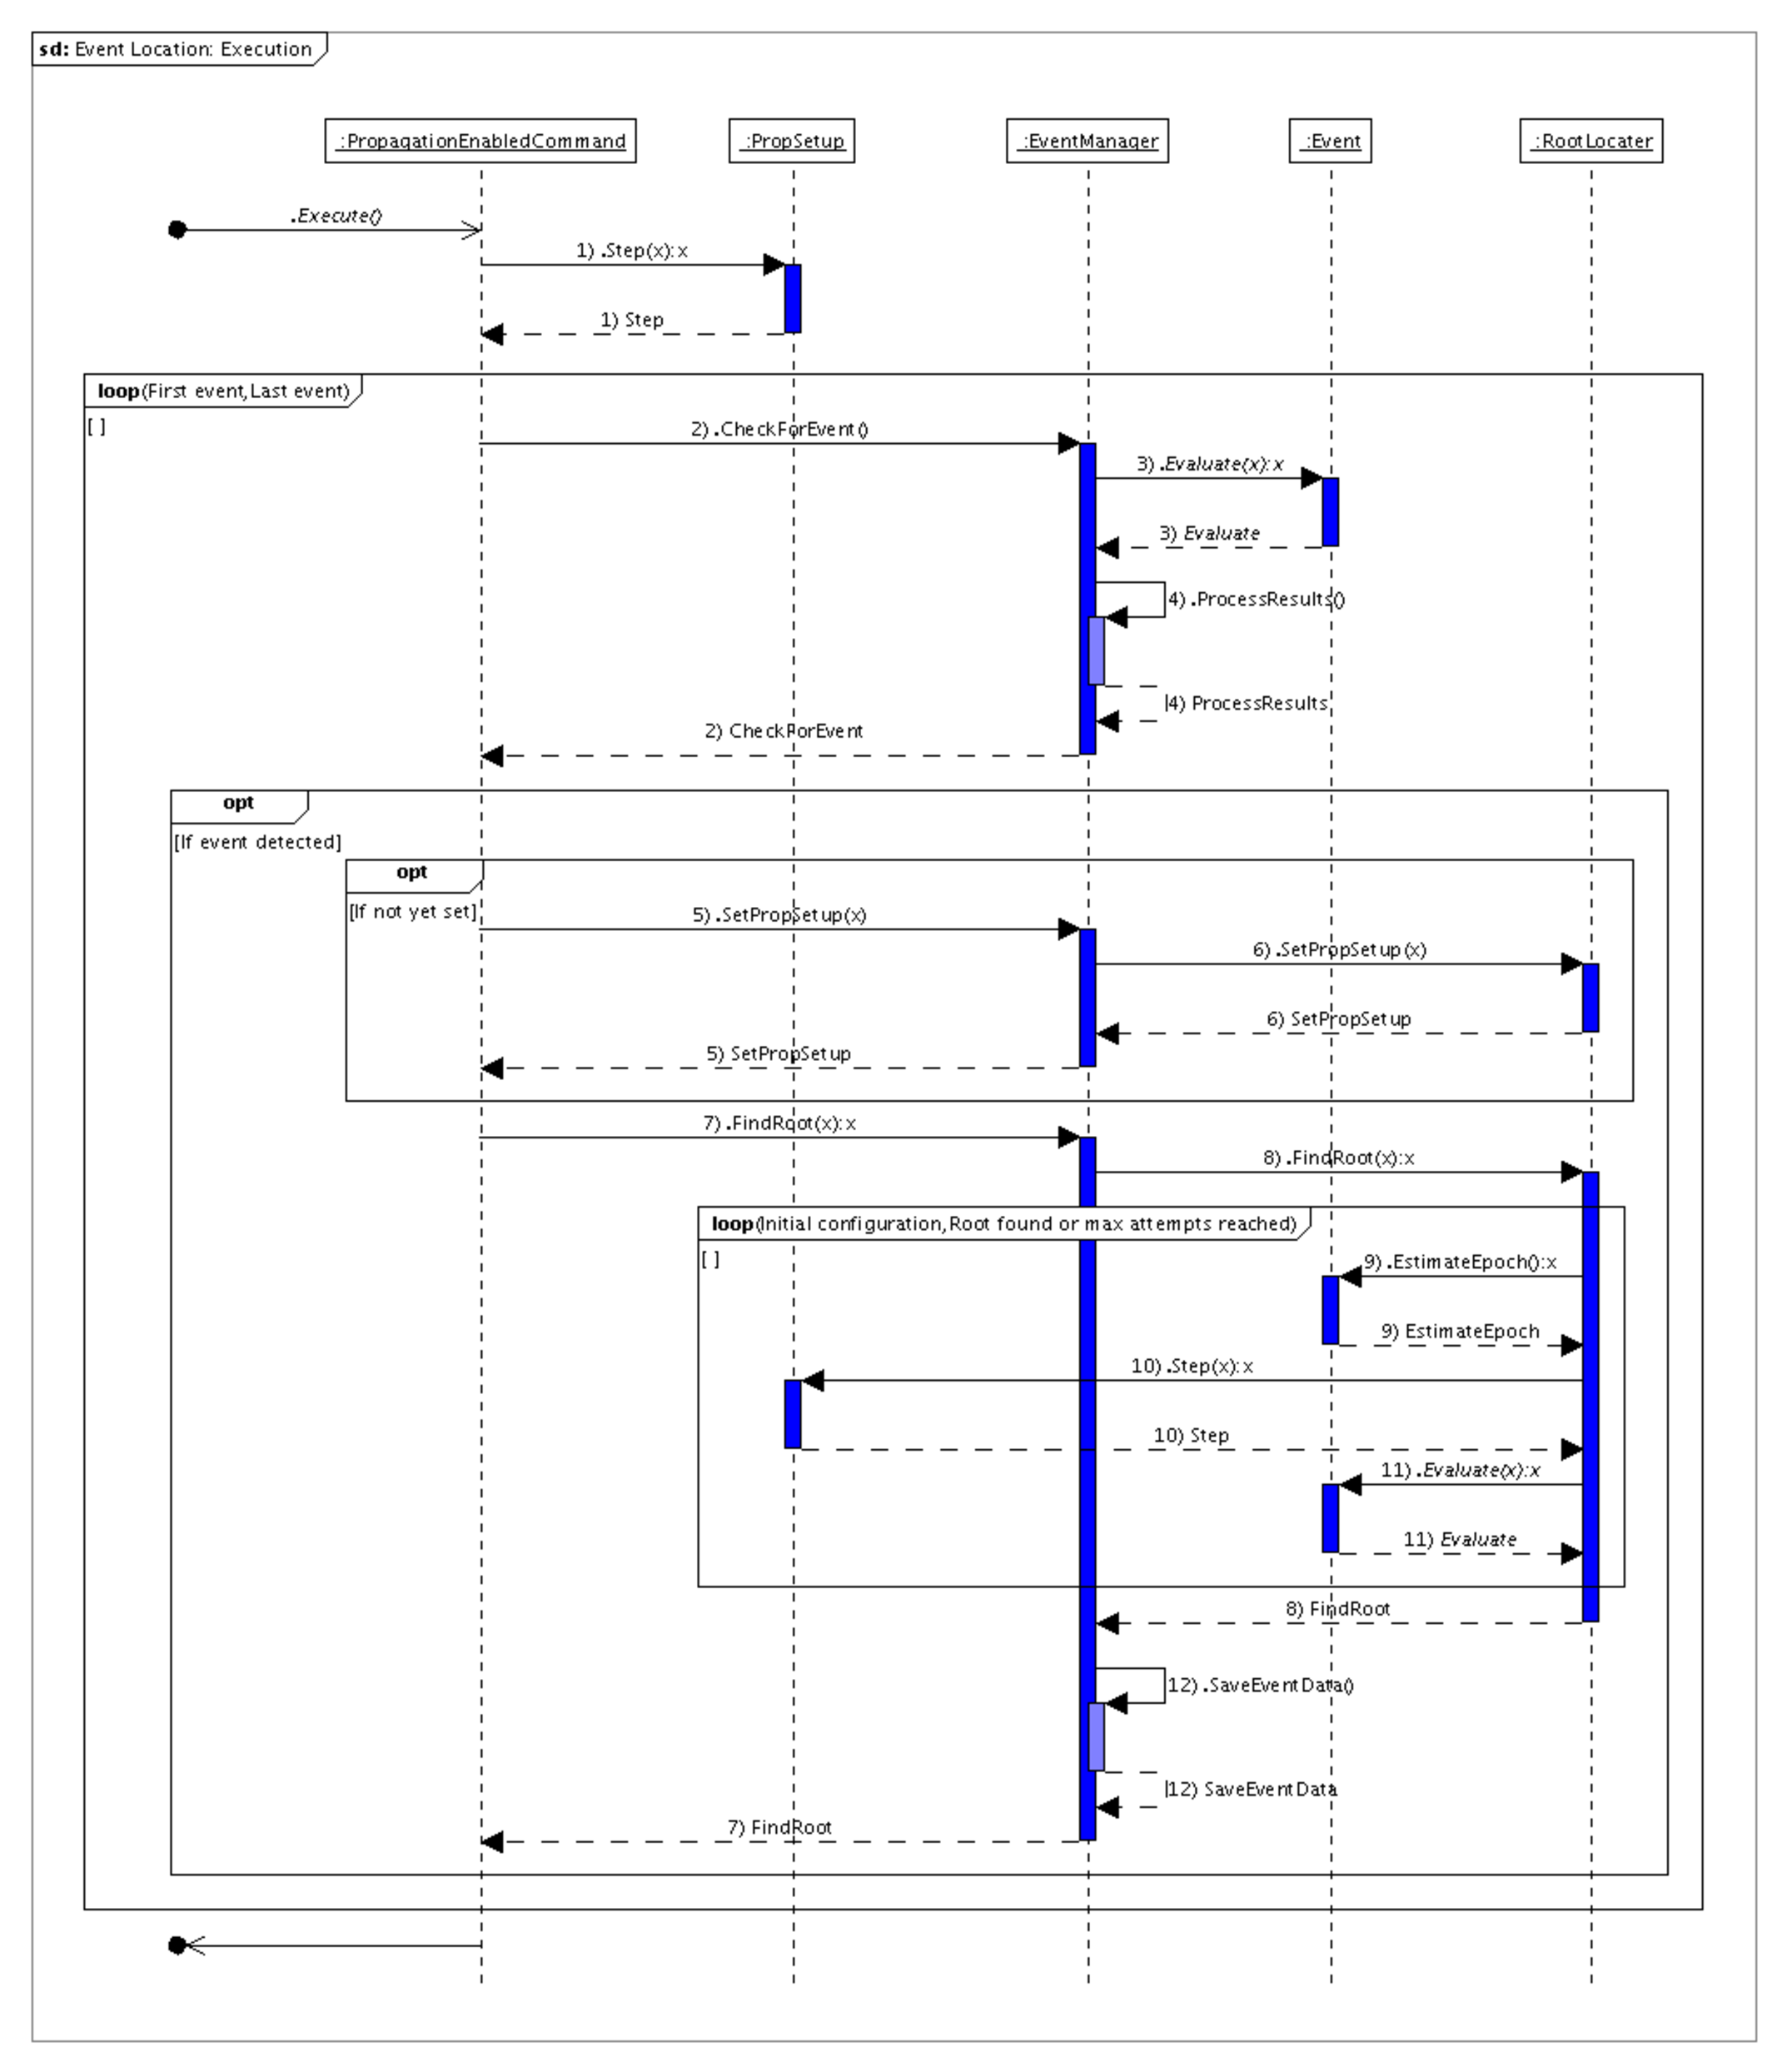
\includegraphics[scale=0.44]{Images/EventLocationExecution.eps}
% EventLocationExecution.png: 1014x1178 pixel, 72dpi, 35.77x41.56 cm, bb=0 0 1014 1178
\caption{\label{fig:EventLocationSD}The Event Location Process}
\end{center}
\end{figure}

If a zero crossing or extremum is detected in the propagation step, the event location code needs to perform additional processing.  This additional processing is controlled by a RootLocator object set during the command's initialization.  If necessary, the RootLocator is passed a pointer to the PropSetup associated with the located event\footnote{Some propagation enabled commands set the PropSetup pointer at initialization; for others, the PropSetup must be set at this point during execution.  The key differentiator for this determination is the relationship of the PropSetup to the other activities performed by the command.  Commands that only use a single PropSetup can set the pointer during initialization, while those that use multiple PropSetups must set the pointer at this point in the process.}.  Control is then handed to the RootLocator responsible for locating the epoch of the detected crossing or extremum through a call to the EventManager's FindRoot() method.

The EventManager buffers the propagated state of the object or objects participating in the event, and then calls the FindRoot() method on a RootLocator configured to work with the event that triggered the search.  The RootLocator performs a series of propagations to epochs inside of the time span covered by the step that triggered the call to FindRoot().  These propagations search for any zero crossings in the propagation interval, and complete when the zero crossings in the interval have been located or when a maximum number of search steps have been performed.  Once this has happened, control is passed to the EventManager, which saves the detected event data, and then returns control to the propagation enabled command.

The event location code uses several classes specialized to the location process.  These new classes, along with key methods implemented in them, are described in the following section.

\section{\label{sec:EventLocationClasses}Event Location Classes}

\begin{figure}
\begin{center}
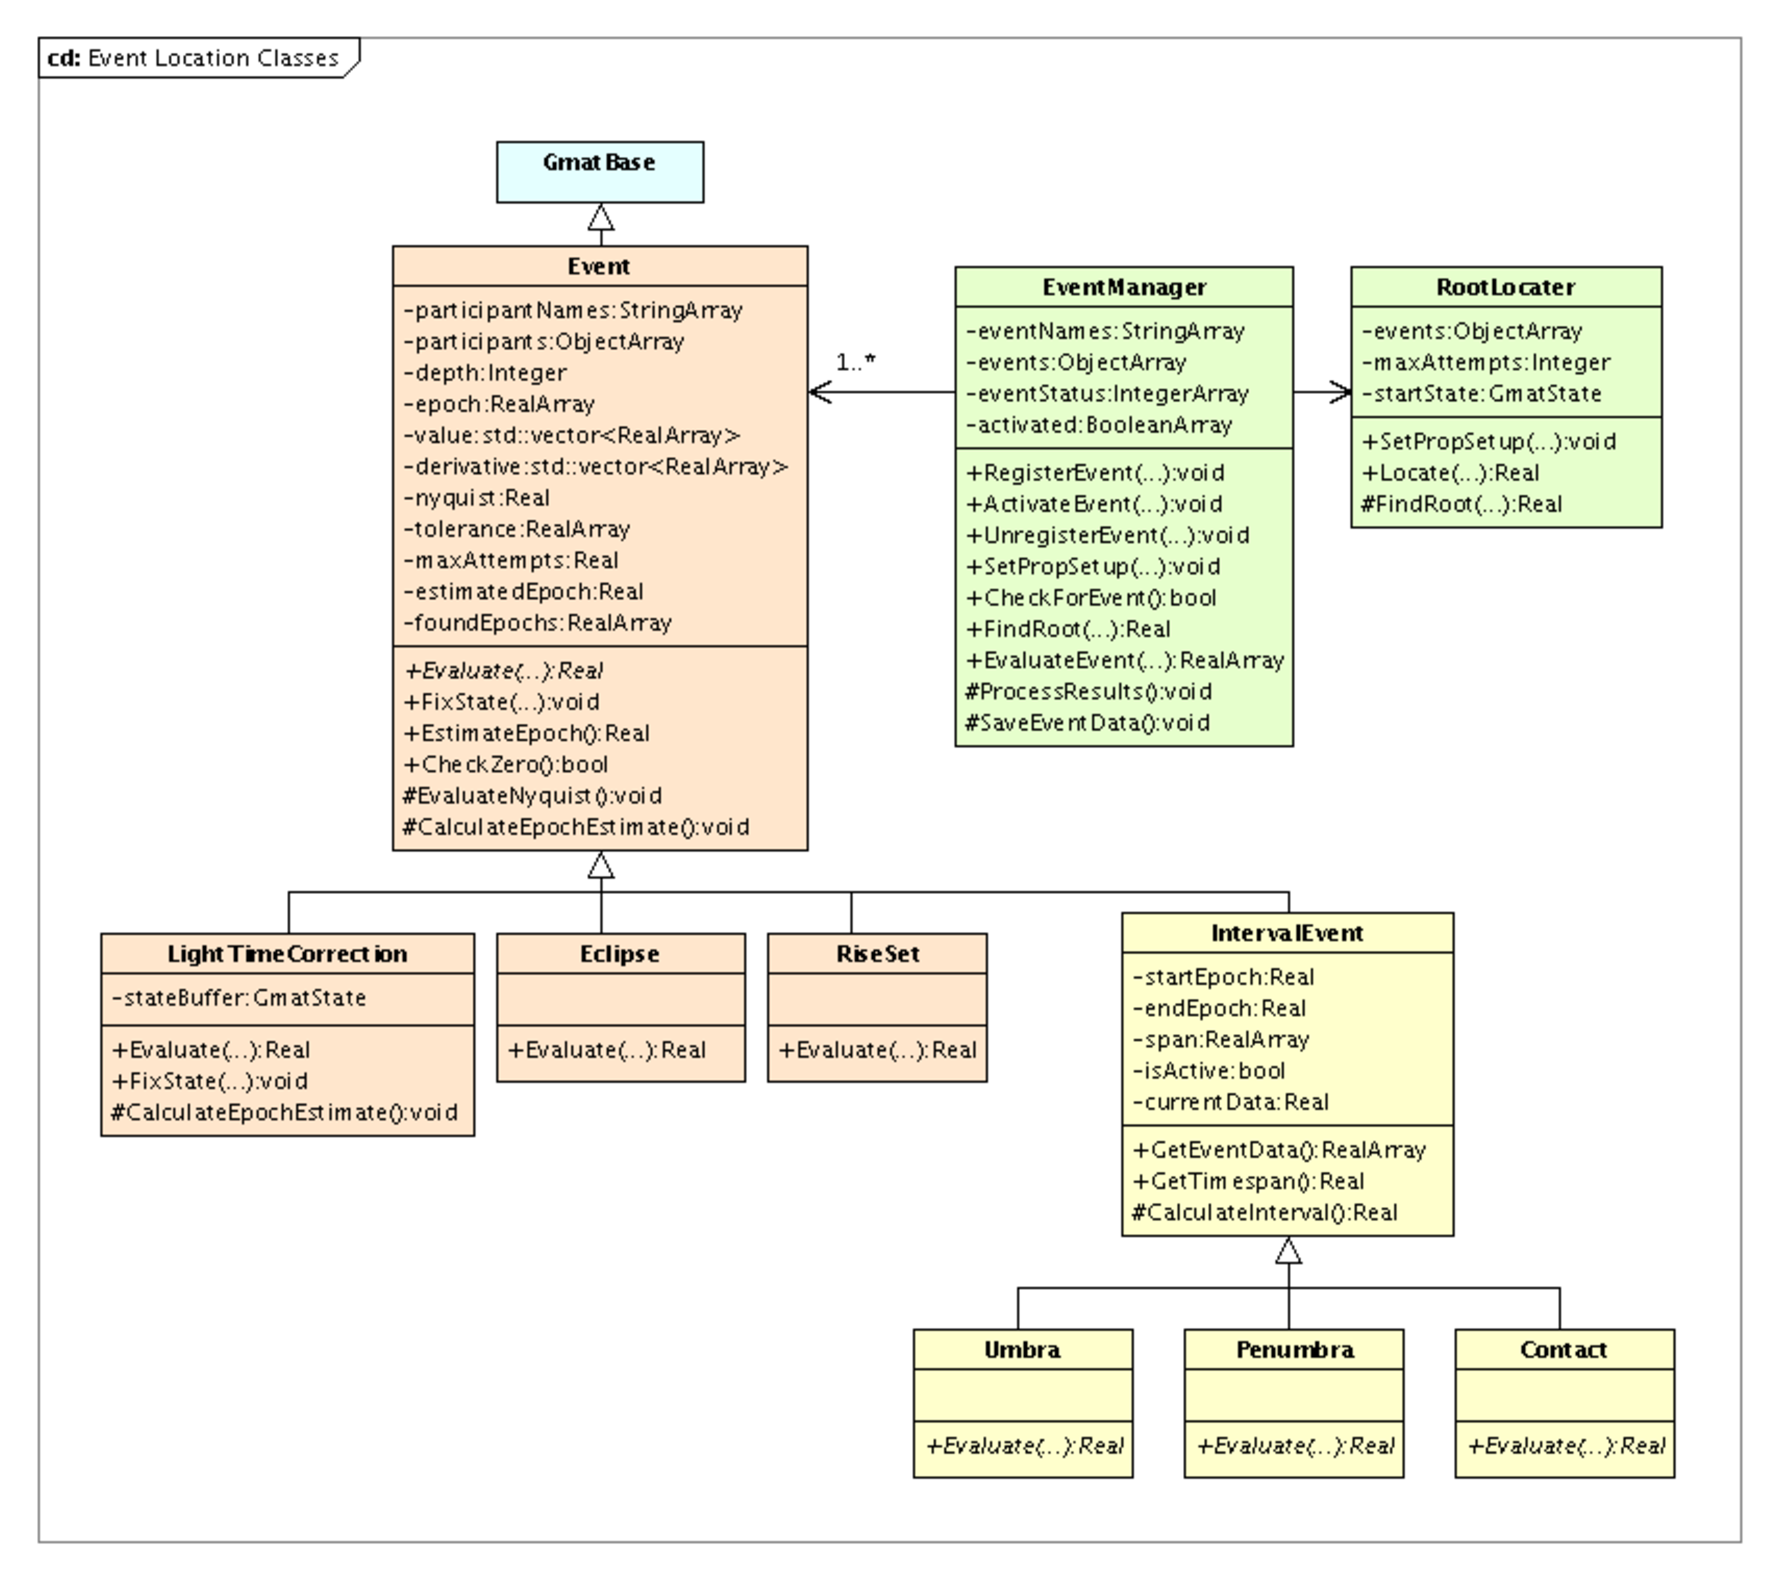
\includegraphics[scale=0.55]{Images/EventLocationClasses.eps}
% EventLocationClasses.png: 837x742 pixel, 72dpi, 29.53x26.18 cm, bb=0 0 837 742
\caption{\label{fig:EventLocationClasses}Event Location Classes}
\end{center}
\end{figure}

Figure~\ref{fig:EventLocationClasses} shows the class relationships between events, the event
manager, and the root finder.  the following paragraphs describe each of these classes in some
detail.

\subsection{Event Classes}

Three specific events are shown in the Figure~\ref{fig:EventLocationClasses}: the RiseSet event, the Eclipse event, and the LightTimeCorrection event.  In addition, the IntervalEvent class and three specific interval events are shown.  In general, event classes are implemented by deriving a class from the Event or IntervalEvent base class, implementing the Evaluate() method to supply event function and derivative data, and if needed, implementing the FixState() method to preserve state data at a specific epoch.  IntervalEvent classes implement additional code used to track the span of the event as well, as is described below.

\subsubsection{The Event Base Class}

All events -- discrete or interval -- are derived from the Event base class.  The Event class provides the interfaces used by the EventManager and RootFinder during the event evaluation process.

\paragraph{Event Attributes}  Each GMAT Event manages its list of objects participating in the event calculation, a ring buffer of the event function values and derivatives, and data identifying the critical frequency (i.e. the Nyquist frequency) specific to the event.  These data are stored in the following data members of the Event class.

\begin{itemize}
\item \textbf{StringArray participantNames}:  Names of the objects that are needed to calculate the event function and derivative information.  These names correspond to objects in the currently running model.
\item \textbf{ObjectArray participants}:  Pointers to the objects that participate in the Event's calculations.
\item \textbf{Integer depth}:  The depth of the ring buffer that tracks the event function values and derivatives.
\item \textbf{RealArray epoch}:  Epoch data for the ring buffer.
\item \textbf{std::vector<RealArray> value}:  Event function vectors for the ring buffer.
\item \textbf{std::vector<RealArray> derivative}:  Event function derivatives for the ring buffer.
\item \textbf{Real nyquist}:  The critical frequency for the event.  This parameter is set to the largest Nyquist frequency in the event; propagation should be performed with step sizes of 1.0/nyquist or smaller in order to catch all of the events in a propagation span.
\item \textbf{Real tolerance}: Numerical tolerance needed for convergence; the event function should evaluate to a magnitude less than this value for located events.
\item \textbf{Real maxAttempts}:  The maximum number of root finding attempts allowed for this event.
\item \textbf{Real estimatedEpoch}:  The estimated epoch for an event, estimaed using the current ring buffer data through a call to EstimateEpoch().
\item \textbf{RealArray foundEpochs}:  The array of event location epochs that have been found.
\end{itemize}

\paragraph{Event Methods}  The Event class inherits code functionality from GmatBase, and
overrides methods as needed to provide Event specific functionality.  The Initialize() method, in particular, is overridden but not listed here since all GmatBase subclasses implement that method when needed.

\begin{itemize}
\item \textbf{Real Evaluate(Integer status) = 0}:  Derived classes implement this method to evaluate the event function and derivative function, filling the resulting data into the epoch, value, and derivative data structures.
\item \textbf{void FixState(GmatBase* obj, bool LockState)}:  Mechanism used to preserve the state data for a specified object -- usually a participant in the event -- for later use in event evaluation.  This method is called when event evaluation requires data at different epochs, so that the data for one object can be preserved prior to propagation, and then accessed at a post-propagation epoch.
\item \textbf{Real EstimateEpoch()}:Provides an estimated a.1 ModJulian epoch for the event.  The estimated epoch is calculated in the CalculateEpochEstimate() method.
\item \textbf{bool CheckZero()}:  Tests to see of the current event function evaluates to an event location, within the specified tolerance.
\item \textbf{void EvaluateNyquist()}:  Method called during initialization to determine the Nyquist frequency for the event.  The Event::Initialize() method calls this protected method.  Derived classes should override this method with their own version of the method if the default Nyquist frequency, 1.0e-99 Hz -- producing basically an unbounded maximum propagation step size -- is not correct.
\item \textbf{void CalculateEpochEstimate()}:  Estimates the epoch of the event based on the event's internal data.  The default implementation uses the data in the ring buffers to interpolate the event epoch.  This method requires that the ring buffer data brackets one or more zero crossings or extrema; events that do not bracket must override this method.
%\item \textbf{}:
\end{itemize}

\subsubsection{Sample Event Subclass: The LightTimeCorrection Class}

The classes derived from the Event class all follow a similar implementation pattern; rather than repeat that pattern in this text, a representative example of a discrete event is presented here.  The LightTimeCorrection class is the most complex of these classes in the figure, so it was selected for this example.

Light-time correction is a calculation that accounts for the finite light propagation time between two participants when calculating a physical quantity.  It is used, for example, when calculating a range measurement to account for the motion of the participants as the ranging signal travels from one to the other.  Since the LightTimeCorrection event needs to preserve state data at one epoch while the RootFinder propagates to a different epoch, it uses both the FixState() method and the Evaluate() method.  The event function for light time correction is the range difference between the light-time calculated distance (that is, the speed of light times the time interval that the signal is in transit), and the range calculated from the state vectors of the participants, where the participant acting as the receiver has its location evaluated at the time the signal is received, and the transmitter's location, at the time the signal left the transmitting participant.

\paragraph{LightTimeCorrection Attributes}

\begin{itemize}
\item \textbf{GmatState stateBuffer}:  The buffer used to temporarily store state data for one participant in the calculation.  For corrections that are tagged with the reception time, the buffer is used to save the state of the receiving participant while the RootFinder propagates backwards to the transmission epoch.
\end{itemize}

\paragraph{LightTimeCorrection Methods}

\begin{itemize}
\item \textbf{Real Evaluate(Integer status)}:  Calculates the event function and its derivatives, as defined in GMAT's mathematical specifications\cite{mathSpec}.
\item \textbf{void FixState(GmatBase* obj, bool lockState)}:  Tells the event to buffer the state of the input object.  lockState is not used in the light time correction, but is supplied to make the method conform to the base class method that is overridden here.
\item \textbf{void CalculateEpochEstimate()}:  Estimates the epoch of a light time endpoint using the range calculated from the participant locations.  This method uses the stateBuffer data as the state of one of the participants for one of the end points, and the current (possibly propagated) state of the other participant as the second endpoint in the calculation.
\end{itemize}

\subsubsection{The IntervalEvent Base Class}

To be written.

\paragraph{IntervalEvent Attributes}

\paragraph{IntervalEvent Methods}

\subsection{The EventManager Class}

Event function monitoring and event location are controlled through the EventManager class.  Each Sandbox contains an EventManager.  The pointer to the local EventManager is passed to each command as the Mission Control Sequence is initialized in the Sandbox.  Commands use this event manager to register, access, evaluate, and locate events as the sequence executes.  The EventManager acts as a mediator between all of the objects in the location process: it tracks the Events and their status, passes PropSetup objects and control to the RootFinder when an event is ready to be located, and passes event function data to any object that needs it.

The sequence diagrams (Figures~\ref{fig:EventLocationSD} and~\ref{fig:MeasurementLocationSD}) show how the EventManager functions in these roles.  The class attributes and methods are described here:

\paragraph{EventManager Attributes}  The core attributes of the EventManger are the data structures that track the Event objects and their status, along with the RootLocator used to find the precise event location.

\begin{itemize}
\item \textbf{StringArray eventNames}:  String descriptions of the events that are registered with the event manager.
\item \textbf{ObjectArray events}:  The current set of Event objects registered with the EventManager.
\item \textbf{RootLocater locater}:  The root locator that searches for event locations once an event has been detected.
\item \textbf{IntegerArray eventStatus}:  The current status of the event.  This event status flag can be set to SEEKING, ZERO\_BRACKETED, EXTREMA\_BRACKETED or LOCATED for each active event.  These values are enumerated in the EventStatus enumeration, a member structure in the EventManager.
\item \textbf{BooleanArray activated}:  Array of flags indicating if the corresponding Event should be checked.  Deactiviated Events are skipped in the evaluation process.
\end{itemize}


\paragraph{EventManager Methods}

\begin{itemize}
\item \textbf{void RegisterEvent(Event newEvent)}:  Adds an event to the EventManager.  When an event is added, it is also evaluated, setting the initial function values on the Event.  Added events are automatically active until deactivated by a call to ActivateEvent().
\item \textbf{void ActivateEvent(Event theEvent, bool makeActive)}:  Sets the activated state for an event.  This call turns on or off event calculations for the specified event, based on the setting of the makeActive flag.  When an inactive event is made active, its ring buffer is cleared and the Evaluate() method is called, providing the initial event function data.  The method is idempotent: activating an active event has no affect, nor does deactivating a deactiveated event.
\item \textbf{void UnregisterEvent(Event theEvent)}:  Removes an event from the event queue.
\item \textbf{void SetPropSetup(Estimator::PropSetup* ps)}:  Sets the PropSetup that will be used for event location.
\item \textbf{bool CheckForEvent()}:  Tests to see if and event has occurred or if an extremum has been encountered.
\item \textbf{Real FindRoot(Integer whichOne)}:  Tells the EventManager to call the RootFinder to locate the specified event.
\item \textbf{RealArray EvaluateEvent(Integer whichOne)}:  Returns the current event function values for the specified event.  This method can be used to retrieve event function data for use in parameters and data subscribers.
\item \textbf{void ProcessResults()}:  Performs processing to determine the event state.
\item \textbf{void SaveEventData()}:  Saves event data so it can be accessed later.
\end{itemize}

\subsection{The RootFinder Class}

Event location in GMAT requires a search over time for a zero of one or more event function values.  The obtained value must fall within a set tolerance of zero; this tolerance is set on each Event object, and defaults to 1.0e-7.  It can be overridden in the Event code.  The RootFinder class performs the search for the function roots.  It works with methods on the Event classes to
retrieve an estimate of the epoch of the root, then drives a PropSetup to move the participants that need propagation to the target epoch.  Finally, it calls the Event's Evaluate() method to determine the current values of the event function, followed by a check for convergence.

The key RootFinder members are described here:

\paragraph{RootFinder Attributes}  The RootFinder uses several internal data structures to manage the root finding process.  These data structures, described here, are transitory; they are only current during the root finding process, and may be stale if examined outside of that process.

\begin{itemize}
\item \textbf{ObjectArray *events}:  The current set of Events that are used to search for roots.
\item \textbf{Integer maxAttempts}:  Maximum number of attempts allowed to find the root.  When maxAttempts is exceeded, the RootFinder posts a message, discards the event location data, and returns.  If a root is located, Events that are being examined because an extremum was detected store the root data, reset the counter, and then search for an additional root.
\item \textbf{GmatState startState}:  The state of all participants at the start of the root search.  This state is restored to the participants at the end of the root finding process.
\end{itemize}

\paragraph{RootFinder Methods}  The root finder uses a propagator set by the EventManager, along with a list of events that may contain roots.  The following methods are used in teh root location process:

\begin{itemize}
\item \textbf{void SetPropSetup(Estimator::PropSetup* ps)}:  Passes a propagator to the root finder.
\item \textbf{Real Locate(ObjectArray \&whichOnes)}:  Public method called by the EventManager to locate all triggered events.  The input ObjectArray contains pointers to all of the Events that need evaluated.  The RootFinder evaluates these events in the order that they are entered into the array.
\item \textbf{Real FindRoot(Event *whichOne)}:  This method is the core root finding code.  It manages all of the propagation and event evaluation needed to find the roots of the event functions.
\end{itemize}
